\documentclass[10pt, titlepage, oneside, a4paper]{article}
\usepackage[T1]{fontenc}
\usepackage[english]{babel}
\usepackage{ifpdf}
\usepackage{amssymb, graphicx, fancyheadings}
\usepackage{rotating}

\addtolength{\textheight}{20mm}
\addtolength{\voffset}{-5mm}
\renewcommand{\sectionmark}[1]{\markleft{#1}}

\def\inst{Computing Science}
\def\typeofdoc{Project Plan}
\def\course{Software Engineering, Spring 2010, 15 hp}
\def\pretitle{Laboration 3}
\def\title{The Greed Game}
\def\namea{Fredrik Dahlberg}
\def\nameb{Marcus Karlsson}
\def\namec{Emil Eriksson}
\def\usernamea{c07fdg}
\def\usernameb{marcusk}
\def\usernamec{c07een}
\def\emaila{\usernamea{}@cs.umu.se}
\def\emailb{\usernameb{}@cs.umu.se}
\def\emailc{\usernamec{}@cs.umu.se}
\def\path{edu/pvt/lab3}
\def\graders{Tor Sterner Johansson}

\def\fullpatha{\raisebox{1pt}{$\scriptstyle \sim$}\usernamea/\path}
\def\fullpathb{\raisebox{1pt}{$\scriptstyle \sim$}\usernameb/\path}
\def\fullpathc{\raisebox{1pt}{$\scriptstyle \sim$}\usernamec/\path}

\begin{document}

	\begin{titlepage}
		\thispagestyle{empty}
		\begin{large}
			\begin{tabular}{@{}p{\textwidth}@{}}
				\textbf{Ume� University \hfill \today} \\
				\textbf{Department of \inst \hfill } \\
				\textbf{\typeofdoc} \\
			\end{tabular}
		\end{large}
		\vspace{10mm}
		\begin{center}
			\LARGE{\pretitle} \\
			\huge{\textbf{\course}}\\
			\vspace{10mm}
			\LARGE{\title} \\
			\vspace{5mm}
			\begin{large}
				\begin{tabular}{ll}
					\textbf{Name} & \namea \\
					\textbf{Email} & \texttt{\emaila} \\
					\textbf{Path} & \texttt{\fullpatha} \\
					\\
					\textbf{Name} & \nameb \\
					\textbf{Email} & \texttt{\emailb} \\
					\textbf{Path} & \texttt{\fullpathb} \\
					\\
					\textbf{Name} & \namec \\
					\textbf{Email} & \texttt{\emailc} \\
					\textbf{Path} & \texttt{\fullpathc} \\
				\end{tabular}
			\end{large}
			\vfill
			\large{\textbf{Grader}}\\
			\mbox{\large{\graders}}
		\end{center}
	\end{titlepage}

	\lfoot{\footnotesize{\usernamea, \usernameb, \usernamec}}
	\rfoot{\footnotesize{\today}}
	\lhead{\sc\footnotesize\title}
	\rhead{\nouppercase{\sc\footnotesize\leftmark}}
	\pagestyle{fancy}
	\renewcommand{\headrulewidth}{0.2pt}
	\renewcommand{\footrulewidth}{0.2pt}

	\pagenumbering{roman}
	\tableofcontents
	
	\newpage

	\pagenumbering{arabic}
	
	\section{Description}
	
		The project aims to create a Greed Game. Greed is a simple turn-based dice game where a player throws a number of dice, receives points and perhaps eventually wins the game when a certain number of points have been accumulated.
	
	\section{Initial design}
	
	\begin{figure}[h]
		\centering
			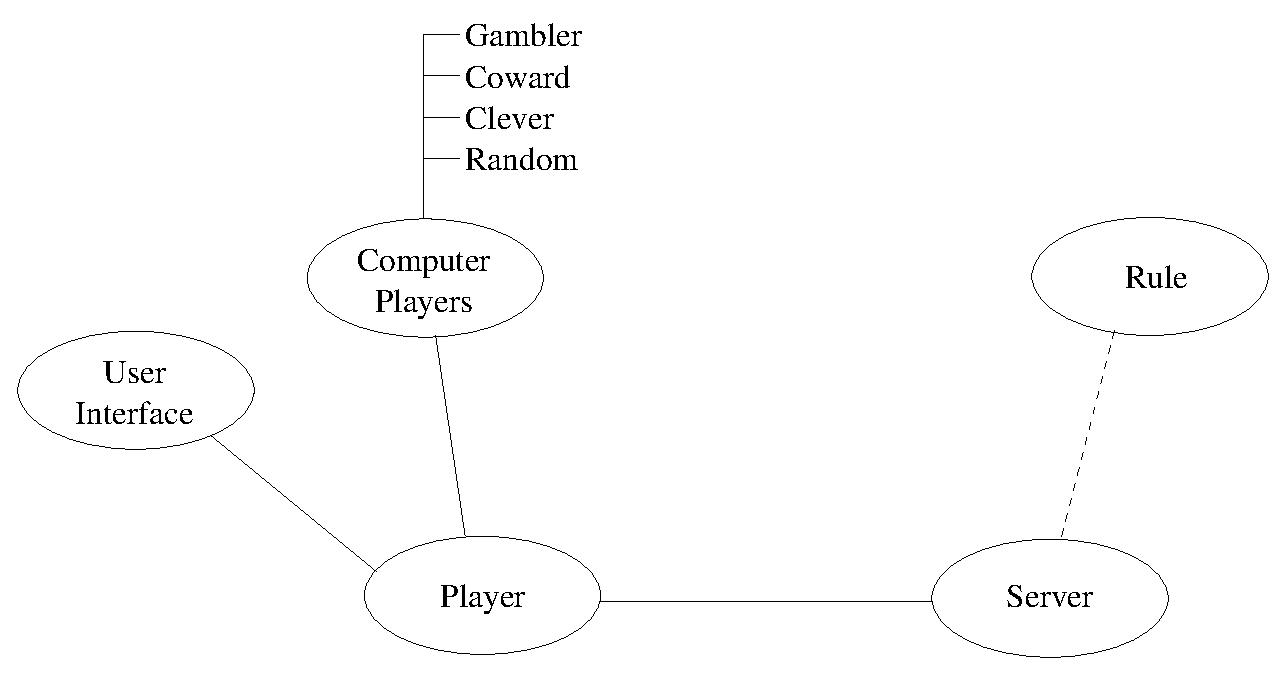
\includegraphics[width=0.8\textwidth]{design.eps}
		\caption{Initial design}
		\label{fig:design}
	\end{figure}
	
	The software will be
	
	\section{Work breakdown}
	
	\begin{table}[t]
		\vspace{15mm}
		\centering
			\begin{tabular*}{0.8\textwidth}{@{\extracolsep{\fill}}l  c c}
				\multicolumn{1}{c}{\begin{rotate}{45}\textbf{Milestone}\end{rotate}} & \begin{rotate}{45}\textbf{Deadline}\end{rotate} & \begin{rotate}{45}\textbf{Estimated} (hrs)\end{rotate}\\
				\hline
				\hline
				Interfaces \& Blackbox tests
					& 2010-03-03 & 6 \\
				Computer Players 
					& 2010-04-06 & 18 \\
				Rules 
					& 2010-04-07 & 6 \\
				Server 
					& 2010-04-09 & 20 \\
				User Interface 
					& 2010-04-13 & 20 \\
				Integration 
					& 2010-04-14 & 6 \\
				\hline
				Project Plan 
					& 2010-03-29 & 20 \\
				Progress Report 
					& 2010-04-08 & 15 \\
				Final Report 
					& 2010-04-15 & 25 \\
					\hline
					\hline
					\textbf{Total estimated time} && 116 \\
					\hline
					\hline
			\end{tabular*}
		\caption{Milestones and time estimations}
		\label{tab:milestones}
	\end{table}
	
		As can be seen in \tablename{} \ref{tab:milestones} (\pagename{} \pageref{tab:milestones}) the work is broken down into several milestones. The "Estimated time"-column is the time estimated to complete each individual milestone.

		\subsection{Schedule}
	\section{Quality assurance}
	
	\section{Tools}

		Ruby has been chosen as the language for implementation. 
	
\end{document}